\documentclass[10pt]{article}

% --- Page geometry (NeurIPS-style) ---
\usepackage[letterpaper,left=1.5in,right=1.5in,top=1in,bottom=1in]{geometry}

% --- Fonts: Times-like ---
\usepackage[T1]{fontenc}
\usepackage[utf8]{inputenc}
\usepackage{amsmath,amsthm}
\usepackage{newtxtext,newtxmath}
\usepackage{microtype}

% --- Math and tables ---
\usepackage{amsfonts,mathtools}
\newtheorem{proposition}{Proposition}
\usepackage{booktabs}
\usepackage{longtable}
\usepackage{array}
\usepackage{tabularx}

% --- Lists ---
\usepackage{enumitem}
\setlist[itemize]{leftmargin=1.5em, itemsep=2pt, topsep=4pt, parsep=0pt}
\setlist[enumerate]{leftmargin=1.6em, itemsep=2pt, topsep=4pt, parsep=0pt}

% --- Colors, graphics, links ---
\usepackage{xcolor}
\usepackage{graphicx}
\usepackage{placeins}
\usepackage{xurl}
\usepackage[hidelinks,unicode]{hyperref}

% --- TikZ and figures ---
\usepackage{tikz}
\usepackage{pgfplots}
\pgfplotsset{compat=1.18}
\usetikzlibrary{arrows.meta,positioning,calc,patterns,decorations.pathreplacing,shapes.geometric}
\usepackage[font=small, labelfont=bf, labelsep=period]{caption}

% --- Paragraph and spacing ---
\setlength{\parindent}{0pt}
\setlength{\parskip}{5.5pt}
\setlength{\emergencystretch}{2em}
\frenchspacing

\urlstyle{same}
\hypersetup{
  pdftitle={Verified Execution for Trust-Explicit Resolution},
  pdfauthor={Andrei Savin}
}

\setcounter{tocdepth}{2}
\setcounter{secnumdepth}{2}

% --- Section formatting (NeurIPS-style) ---
\usepackage{titlesec}
\titleformat{\section}{\normalfont\large\bfseries}{\thesection}{0.6em}{}
\titleformat{\subsection}{\normalfont\normalsize\bfseries}{\thesubsection}{0.6em}{}
\titleformat{\subsubsection}{\normalfont\normalsize\itshape}{\thesubsubsection}{0.5em}{}
\titlespacing*{\section}{0pt}{10pt plus 2pt minus 2pt}{4pt plus 1pt minus 1pt}
\titlespacing*{\subsection}{0pt}{8pt plus 2pt minus 2pt}{3pt plus 1pt minus 1pt}
\titlespacing*{\subsubsection}{0pt}{6pt plus 2pt minus 1pt}{2pt plus 1pt minus 1pt}

% --- Page style: just page numbers ---
\pagestyle{plain}

% --- Abstract environment (NeurIPS-style) ---
\renewenvironment{abstract}{%
  \centerline{\bfseries\normalsize Abstract}%
  \vspace{0.5ex}%
  \begin{quote}\small
}{%
  \end{quote}%
}

% --- Helpers ---
\newcolumntype{Y}{>{\raggedright\arraybackslash}X}

\begin{document}

\begin{center}
{\LARGE\bfseries Verified Execution for Trust-Explicit Resolution\par}
\vspace{0.4em}
{\large Merkle Traces, Attested Runners, and the Two-Axis Trust Model\par}
\vspace{1.2em}
{\normalsize\bfseries Andrei Savin\par}
\vspace{0.3em}
{\small question.market\par}
{\small\href{mailto:andrei@andreisavin.com}{andrei@andreisavin.com}\par}
\vspace{0.6em}
{\small April 2026; revised October 2026\par}
\end{center}

\vspace{0.8em}

\begin{abstract}
A market that commits to an executable resolution blueprint has declared what the resolver should do. It has not established that the resolver did it. A proposer can fabricate a trace, or run a valid stochastic procedure repeatedly and submit only the favorable result. Both attacks survive a superficially convincing execution record.

This paper defines a progressive verification stack for closing that gap. A two-axis trust model separates the kind of judgment used to resolve a market from the evidence supporting its execution. A bounded reference protocol gives exact canonical encodings, count-bound Merkle commitments, complete trace semantics, authenticated source inputs, and publication before the challenge clock starts. Independent runners commit separately to their own evidence while agreeing on a shared request-bound result. We prove commitment binding, trace consistency, publication gating, quorum conditions, and the limits and remedies of selective execution. A compositional theorem permits different steps to use replay, proofs, or attestation without hiding their boundary assumptions.

The revision evaluates these claims with adversarial protocol tests, independent Python and JavaScript commitment implementations, exact committee analysis, seeded selection experiments, and compiled Algorand verifier measurements. Signed and TEE-attested runners strengthen provenance; source authentication, authorized attempts, and funded challenges remain necessary. The central claim is concrete: markets should not only commit to a decision program, but progressively improve evidence that the committed program actually ran.
\end{abstract}
\vspace{1em}
{\small\renewcommand{\contentsname}{}\setcounter{tocdepth}{2}\tableofcontents}
\vspace{0.5em}
\section{Introduction}

Resolution is where trust concentrates in prediction markets. A market can make its pricing, accounting, and settlement rules executable. It must still connect those rules to something that happened outside the contract. The question is not whether trust is required, but whether it is visible.

The companion paper on trust-explicit resolution \cite{trustexplicit2026} proposes that every market carry an executable resolution constitution: declared sources, judgment steps, decision rules, dispute paths, and funding. That fixes what the resolver is supposed to do. The next question is simpler: how does anyone know the resolver did it?

A proposer can fabricate a plausible trace, submit a bonded result, and bet that nobody will check. A signature identifies who endorsed that claim. A hash prevents later editing. Neither alone establishes that the declared program ran. This is the execution integrity gap. It is distinct from the truth problem. An authentic runner can faithfully process a false source report. A fabricated execution can accidentally produce the right answer. Both distinctions matter when money settles on the result.

This paper closes parts of that gap with a progressive verification stack:
\begin{enumerate}
\item \textbf{Blueprint commitment} fixes the decision program and its fallback rules before trading.
\item \textbf{Trace commitment and publication} fix a complete, inspectable account of the claimed run and make individual disputes compact.
\item \textbf{Execution assurance} binds that account to a runner identity, an attested execution environment, or a committee with an explicit fault model.
\item \textbf{Economic fallback} funds the checking and adjudication that remain necessary outside those guarantees.
\end{enumerate}

The stack also needs a common execution request. It binds the market, blueprint, source snapshot, permitted attempts, and acceptance policy. Otherwise a perfectly attested runner can repeatedly execute a stochastic workflow and submit whichever result it likes. Verifying an invocation is not enough. The protocol must verify that this was an authorized invocation and account for attempts that disappeared.

\begin{figure}[t]
\centering
\resizebox{0.98\linewidth}{!}{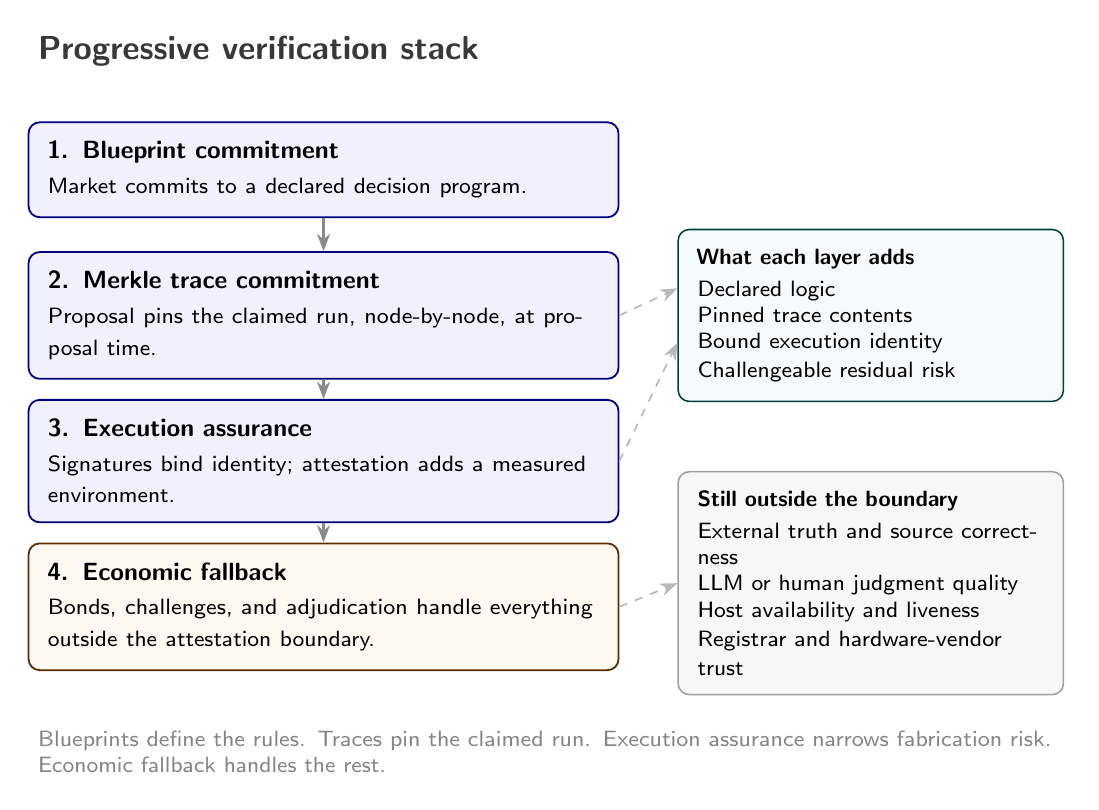
\begin{tikzpicture}[
  x=1cm, y=1cm,
  every node/.style={font=\sffamily},
  >={Stealth[length=2.2mm]},
  % ── Main stack layers ────────────────────────────────────────────
  layer/.style={
    text width=7cm, minimum height=1.2cm,
    align=left, inner sep=7pt,
    rounded corners=4pt, line width=0.65pt,
    font=\sffamily\fontsize{9.5pt}{11.5pt}\selectfont,
  },
  qcore/.style={layer, draw=blue!50!black, fill=blue!6},
  qecon/.style={layer, draw=orange!35!black, fill=orange!5},
  % ── Side annotations ────────────────────────────────────────────
  annot/.style={
    text width=4.4cm, minimum height=1.2cm,
    align=left, inner sep=7pt,
    rounded corners=4pt, line width=0.55pt,
    font=\sffamily\fontsize{8.5pt}{10.5pt}\selectfont,
  },
  qadds/.style={annot, draw=teal!50!black, fill=teal!4},
  qout/.style={annot, draw=black!38, fill=black!3},
  % ── Misc ─────────────────────────────────────────────────────────
  note/.style={
    font=\sffamily\fontsize{7.8pt}{9.5pt}\selectfont,
    text=black!48, align=left, text width=13cm,
  },
  ftitle/.style={
    font=\sffamily\bfseries\fontsize{13pt}{14.5pt}\selectfont,
    text=black!78,
  },
  flow/.style={->, line width=0.85pt, draw=black!46},
  conn/.style={->, line width=0.6pt, draw=black!28, dashed},
]

% ── Title ──────────────────────────────────────────────────────────
\node[anchor=west, ftitle] at (0, 0.5) {Progressive verification stack};

% ── Stack layers ───────────────────────────────────────────────────
\node[qcore] (L1) at (3.75, -1.0) {%
  \textbf{1.\enspace Blueprint commitment}\\[1pt]
  {\footnotesize Market commits to a declared decision program.}};

\node[qcore] (L2) at (3.75, -2.85) {%
  \textbf{2.\enspace Merkle trace commitment}\\[1pt]
  {\footnotesize Proposal pins the claimed run, node-by-node, at proposal time.}};

\node[qcore] (L3) at (3.75, -4.7) {%
  \textbf{3.\enspace Execution assurance}\\[1pt]
  {\footnotesize Signatures bind identity; attestation adds a measured environment.}};

\node[qecon] (L4) at (3.75, -6.55) {%
  \textbf{4.\enspace Economic fallback}\\[1pt]
  {\footnotesize Bonds, challenges, and adjudication handle everything outside the attestation boundary.}};

% ── Vertical flow ─────────────────────────────────────────────────
\draw[flow] (L1) -- (L2);
\draw[flow] (L2) -- (L3);
\draw[flow] (L3) -- (L4);

% ── Side: what each layer adds ────────────────────────────────────
\node[qadds] (adds) at (10.7, -2.85) {%
  \textbf{What each layer adds}\\[2pt]
  {\footnotesize
  Declared logic\\
  Pinned trace contents\\
  Bound execution identity\\
  Challengeable residual risk}};

% ── Side: still outside ───────────────────────────────────────────
\node[qout] (outside) at (10.7, -6.25) {%
  \textbf{Still outside the boundary}\\[2pt]
  {\footnotesize
  External truth and source correctness\\
  LLM or human judgment quality\\
  Host availability and liveness\\
  Registrar and hardware-vendor trust}};

% ── Connecting arrows (split targets to avoid overlap) ────────────
\draw[conn] (L2.east) -- (adds.172);
\draw[conn] (L3.east) -- (adds.188);
\draw[conn] (L4.east) -- (outside.west);

% ── Bottom note ────────────────────────────────────────────────────
\node[note, anchor=north west] at (0, -8.0) {%
  Blueprints define the rules. Traces pin the claimed run.
  Execution assurance narrows fabrication risk.
  Economic fallback handles the rest.};

\end{tikzpicture}
}
\caption{Progressive verification. The execution request, publication gate, and challenge policy bind the layers into one resolution procedure.}
\label{fig:stack}
\end{figure}

\subsection{Contributions}

Markets should progressively improve the evidence that their committed decision program actually ran. This paper gives that thesis a concrete protocol and a set of testable claims.

First, the two-axis trust model separates \emph{what kind of judgment determines the outcome} from \emph{what supports the execution claim}. A deterministic source rule with anonymous execution and an LLM judgment with attested execution have different risks. A single trust score obscures that distinction.

Second, a bounded reference protocol specifies canonical bytes, a count-bound Merkle tree, complete trace semantics, authenticated source objects, and a publication state machine. We prove what an accepted trace establishes and give explicit omission and forgery counterexamples for weaker checks. The protocol uses a full-trace hash as its baseline: Merkle structure adds compact authenticated openings, not a new guarantee that the original account was honest.

Third, we separate each runner's evidence receipt from the shared result on which a committee agrees. We derive quorum safety, liveness, trust-domain constraints, and attempt-selection bounds. These identify exactly when replication strengthens assurance and when it merely repeats the same dependency.

Finally, executable adversarial tests, independent commitment implementations, exact committee enumeration, seeded selection experiments, and compiled AVM measurements exercise the repaired design. The research artifacts are independent of question.market's current implementation. They establish properties of the declared research protocol, with hardware deployment and field behavior left as separately specified experiments.

\subsection{Related work and current direction}

\textbf{Declared resolution and disputes.} Optimistic oracles and bonded-answer systems make a claim contestable. The companion paper supplies the dispute economics and declared workflow for this design \cite{trustexplicit2026}. Here the object being contested is the execution of that workflow. We do not assume that the presence of a bond guarantees an attentive verifier.

\textbf{Authenticated computation and fraud proofs.} Town Crier supplies TEE-backed authenticated data feeds; Ekiden separates confidential execution from consensus \cite{towncrier2016,ekiden2019}. Arbitrum's optimistic computation makes incorrect off-chain execution claims subject to narrow on-chain disputes \cite{arbitrum2018}. Our local trace challenges use this established separation between a commitment and a proof of an invalid transition. A Merkle inclusion proof authenticates the disputed record; a semantic check establishes the fault.

\textbf{Replicated confidential execution.} Chainlink Confidential Compute already specifies replicated enclaves, result comparison, and threshold-generated deterministic randomness; it also describes a ZK execution tier \cite{chainlinkcc}. The contribution here is not the invention of replicated TEEs. It is a market-resolution protocol that binds requests, attempts, complete evidence, quorum composition, and disputes to the constitution chosen before trading.

\textbf{Attestation and release transparency.} The RATS architecture distinguishes the attester, verifier, and relying party \cite{rats2023}. This maps naturally to the enclave, registrar, and market contract. Apple's Private Cloud Compute requires attested measurements to appear in a public release-transparency log \cite{pcc2026}. That is a useful precedent for making the source-to-measurement mapping inspectable instead of treating a measurement as an unexplained allowlist entry.

\textbf{Source and model provenance.} DECO and TLSNotary address evidence of data obtained from authenticated TLS sources \cite{deco2020,tlsnotary}. AEX, a March 2026 preprint, studies signed provenance across LLM API intermediaries and explicitly distinguishes endpoint accountability from proof of model inference \cite{aex2026}. An August 2026 technical note combines action evidence with RATS-style attestation in an emulated TPM experiment \cite{aep2026}. These are relevant developing directions, not demonstrations that a remotely hosted model executed inside this paper's runner enclave.

\textbf{Proofs and persistent state.} zkLLM demonstrates that proving substantial model computation is a concrete research program, making a blanket claim that ZK execution is infeasible untenable \cite{zkllm2024}. Rollback-resistant storage work likewise shows why protected execution memory does not by itself supply persistent one-shot state \cite{teerex2026}. This design therefore places request authorization and attempt consumption in an authoritative ledger, and treats proof-carrying deterministic subgraphs as a promising extension.

\section{The Two-Axis Trust Model}
\label{sec:twoaxis}

The resolution class describes the decision program:
\begin{itemize}
\item \textbf{Source-based}: declared computations over external or on-chain records, without model-mediated or human judgment.
\item \textbf{Agent-assisted}: at least one model-mediated judgment. A fixed local model with fixed decoding can be deterministic; determinism does not remove its judgment role.
\item \textbf{Human-judged}: at least one human decision. Recorded testimony can be replayed as an input even when the underlying judgment cannot be recomputed.
\end{itemize}
When a workflow mixes classes, its displayed primary label gives human judgment precedence over model judgment over source processing, while retaining the full list of dependencies. This is a display convention, not an ordering of safety.

Execution assurance describes the support for a particular submitted claim:
\begin{itemize}
\item \textbf{Unauthenticated}: a commitment fixes the account, without an approved execution identity.
\item \textbf{Signed runner}: an authorized key endorses the request-bound receipt.
\item \textbf{TEE-attested}: an appraised hardware attestation binds that key to an approved measured environment under a declared registration policy.
\item \textbf{Threshold TEE-attested}: an eligible committee supplies a certificate satisfying explicit signer and trust-domain rules.
\end{itemize}
The four named modes give twelve descriptive combinations with the three resolution classes. They are not a theorem that risks are statistically independent, nor a universal ladder on which every larger committee is safer. Replayability, input authentication, selection policy, availability, and shared trust dependencies remain visible descriptors.

\begin{figure}[t]
\centering
\resizebox{0.98\linewidth}{!}{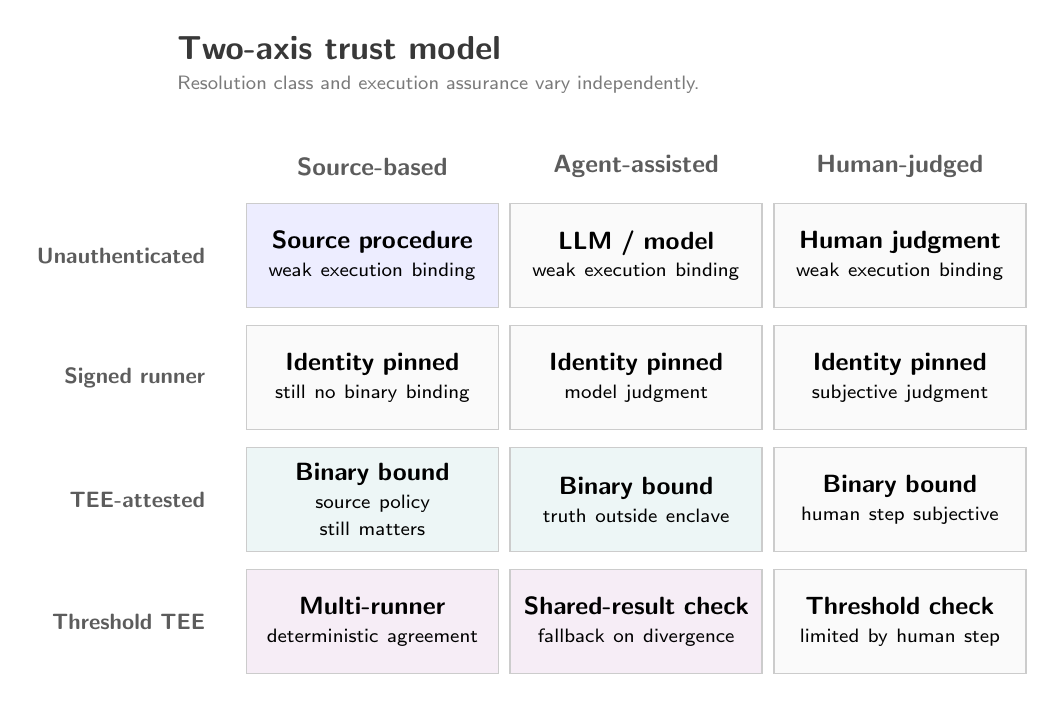
\begin{tikzpicture}[
  x=1cm, y=1cm,
  every node/.style={font=\sffamily},
  % ── Typography ───────────────────────────────────────────────────
  ftitle/.style={
    font=\sffamily\bfseries\fontsize{12.8pt}{13.8pt}\selectfont,
    text=black!78,
  },
  axislbl/.style={
    font=\sffamily\bfseries\fontsize{8.9pt}{9.9pt}\selectfont,
    text=black!68,
  },
  rowhead/.style={
    font=\sffamily\bfseries\fontsize{8.4pt}{9.4pt}\selectfont,
    text=black!64, align=right,
  },
  colhead/.style={
    font=\sffamily\bfseries\fontsize{8.6pt}{9.6pt}\selectfont,
    text=black!64, align=center,
  },
  small/.style={
    font=\sffamily\fontsize{7.3pt}{8.2pt}\selectfont,
    text=black!52, align=center,
  },
  % ── Grid cells ───────────────────────────────────────────────────
  cell/.style={
    draw=black!20, line width=0.55pt,
    minimum width=3.15cm, minimum height=1.32cm,
    text width=2.85cm,
    align=center, inner sep=5pt,
    font=\sffamily\fontsize{8.7pt}{10pt}\selectfont,
  },
  hi1/.style={cell, fill=blue!7},
  hi2/.style={cell, fill=teal!7},
  hi3/.style={cell, fill=violet!7},
  base/.style={cell, fill=black!2},
]

% ── Title ──────────────────────────────────────────────────────────
\node[anchor=west, ftitle] at (-0.05, 0.78) {Two-axis trust model};
\node[anchor=west, small] at (-0.05, 0.32) {Resolution class and execution assurance vary independently.};

% ── Column headers ─────────────────────────────────────────────────
\node[colhead] at (2.55, -0.72) {Source-based};
\node[colhead] at (5.90, -0.72) {Agent-assisted};
\node[colhead] at (9.25, -0.72) {Human-judged};

% ── Row headers ────────────────────────────────────────────────────
\node[rowhead, anchor=east] at (0.55, -1.85)  {Unauthenticated};
\node[rowhead, anchor=east] at (0.55, -3.40) {Signed runner};
\node[rowhead, anchor=east] at (0.55, -4.95)  {TEE-attested};
\node[rowhead, anchor=east] at (0.55, -6.50) {Threshold TEE};

% ── Row 1: Unauthenticated ────────────────────────────────────────
\node[hi1]  at (2.55, -1.85)  {\textbf{Source procedure}\\{\scriptsize weak execution binding}};
\node[base] at (5.90, -1.85)  {\textbf{LLM / model}\\{\scriptsize weak execution binding}};
\node[base] at (9.25, -1.85)  {\textbf{Human judgment}\\{\scriptsize weak execution binding}};

% ── Row 2: Signed runner ──────────────────────────────────────────
\node[base] at (2.55, -3.40) {\textbf{Identity pinned}\\{\scriptsize still no binary binding}};
\node[base] at (5.90, -3.40) {\textbf{Identity pinned}\\{\scriptsize model judgment}};
\node[base] at (9.25, -3.40) {\textbf{Identity pinned}\\{\scriptsize subjective judgment}};

% ── Row 3: TEE-attested ───────────────────────────────────────────
\node[hi2]  at (2.55, -4.95)  {\textbf{Binary bound}\\{\scriptsize source policy still matters}};
\node[hi2]  at (5.90, -4.95)  {\textbf{Binary bound}\\{\scriptsize truth outside enclave}};
\node[base] at (9.25, -4.95)  {\textbf{Binary bound}\\{\scriptsize human step subjective}};

% ── Row 4: Threshold TEE ──────────────────────────────────────────
\node[hi3]  at (2.55, -6.50) {\textbf{Multi-runner}\\{\scriptsize deterministic agreement}};
\node[hi3]  at (5.90, -6.50) {\textbf{Shared-result check}\\{\scriptsize fallback on divergence}};
\node[base] at (9.25, -6.50) {\textbf{Threshold check}\\{\scriptsize limited by human step}};

\end{tikzpicture}
}
\caption{The two axes describe different facts. Replayability additionally depends on the input snapshot and runtime; a model-based decision can be deterministic, and an unsigned live source can be impossible to replay.}
\label{fig:twoaxis}
\end{figure}

For market $M$, blueprint $G$, proposal $P$, and ledger time $t$, write
\[
\mathcal T(M,P,t)=\bigl(\kappa(G),\epsilon_{\rm req}(M),
\epsilon_{\rm run}(P,t),\rho,\sigma,\eta,\mathcal D\bigr).
\]
Here $\rho$ records replayability and source authentication, $\sigma$ the attempt-selection rule, $\eta$ publication and fallback policy, and $\mathcal D$ the dependency graph of operators, registrars, vendors, builds, and sources. The market declares a required mode at creation. The realized mode is checked against the receipt and current registry; an expired key or unavailable quorum cannot silently downgrade it.

The profile is descriptive, not prescriptive. It tells participants what they are relying on. A participant can prefer a transparent deterministic source computation to an attested subjective judgment without pretending that the latter's execution evidence is worthless. Trust becomes visible enough to price.

\section{Security Model and Protocol Objects}
\label{sec:model}

The adversary can operate the proposer and host, choose when to send messages, withhold evidence, restart processes, control allowed faulty committee members, and corrupt declared trust domains. It can supply arbitrary traces and unauthenticated network bytes. It cannot forge an honest source or runner signature, find hash collisions, or change finalized ledger state under the corresponding cryptographic and ledger assumptions. TEE claims additionally assume the declared hardware and measured-code boundaries hold. These assumptions are separate: a broken registrar can defeat an otherwise intact enclave.

The adversary's objectives are to finalize an outcome inconsistent with the declared computation, conceal a required input or step, substitute an unauthorized execution, select a favorable stochastic result, or block resolution. Source falsity and poor judgment are distinct objectives handled by source policy and adjudication. A valid execution proof is compatible with a wrong real-world answer.

\subsection{One request, distinct evidence receipts}

Before execution, an authoritative request fixes the chain and market identity, blueprint and semantics version, input-snapshot commitment, permitted attempt policy, authorized runners, timing, and publication rule. Its identifier $q$ is a domain-separated digest of the canonical request. The snapshot fixes the exact source objects or the rule by which independently authenticated objects become fixed; a URL and a loose time window alone do not identify common input bytes.

Runner $j$ produces its own receipt $E_j$, binding $q$, its run identity and measurement, the complete trace root and count, and the shared result digest $d$. The common result contains $q$ and the declared terminal output. It excludes run-specific timestamps, trace locations, keys, and measurements. In a committee, every signature binds both $d$ and $E_j$:
\[
\operatorname{Sig}_{K_j}\!\left(H(\mathrm{domain},d,E_j)\right).
\]
The concrete encoding is versioned; this notation denotes an unambiguous typed object, not raw concatenation of variable-length fields. An authorized receipt may have a different root from another receipt while endorsing the same result. That difference is expected, not evidence of dishonesty.

Agreement is meaningful only over the same $q$. For deterministic computation, identical authenticated inputs and semantics imply identical terminal results. For a stochastic or human step, the constitution must define fixed aggregation or a fallback on divergence. Deterministic descendants are compared conditional on equal parent inputs. Two honest computations fed different judgments need not agree merely because their later nodes are deterministic.

\subsection{Two different claims}

A complete trace plus successful replay establishes that the declared result is consistent with the declared computation over the recorded inputs. It does not establish the historical fact that the original proposer performed that work. An execution receipt can add provenance under its assurance assumptions. Neither fact establishes the truth of an external report.

Keeping these claims separate makes verification stronger. The protocol can reject a fabricated, inconsistent trace without asking which machine produced it. It can accept a consistent computation while exposing the precise source or judgment on which its conclusion rests. And it can demand stronger provenance when a market's constitution makes actual invocation, model identity, or exclusive key custody material.

\section{Complete Traces and Compact Challenges}
\label{sec:merkle}

The reference profile deliberately fixes a small executable language so every acceptance rule can be tested. A blueprint has between 4 and 64 ordered slots: an authenticated integer source, zero or more additions of one, one comparison against the declared slot count, and two mutually exclusive Boolean terminals. Both terminal slots appear in the trace; the unselected one is explicitly skipped. The blueprint hash authenticates the exact grammar, constants, source policy, slot count, and semantics version. This profile exercises data flow, branching, source authentication, omission, and terminal linkage. The compositional theorem in Section~\ref{sec:composition} states the extension to arbitrary acyclic graphs; the prototype does not pretend to implement that entire language.

\subsection{Canonical objects and exact tree construction}

The public protocol specification and vectors are part of the paper's reproducibility package. Objects use a restricted canonical JSON profile: ASCII strings and keys, exact integers of magnitude at most $2^{53}-1$, booleans, null, arrays, and objects; sorted object keys; no insignificant whitespace; duplicate keys, floating-point spellings, unknown schema fields, and noncanonical encodings are rejected. Large external values are represented by explicitly typed byte or decimal encodings before entering the profile. There is no implicit Unicode normalization or approximate numeric coercion. This avoids claiming that a default JSON serializer implements all of RFC~8785, whose full number and Unicode rules are more demanding \cite{rfc8785}.

Let $J(x)$ be the canonical bytes and let $H$ be SHA-256. For an object domain $D$, define $H_D(x)=H(D\|\mathtt{00}\|J(x))$. Domains are ASCII constants without zero bytes. The source report, blueprint, request, run context, semantic projection, and terminal result have distinct domains. Hash digests are raw 32-byte values inside the binary tree envelopes and lowercase 64-character hexadecimal strings in JSON. A consumer obtains the schema version from the authenticated object or protocol context, not by trying to read a domain tag out of a bare digest.

The per-run context commitment $C$ includes the request and snapshot digests, run identity, runner identity, and measurement. For record bytes $B_i$, a count $n$, and zero-based position $i$, the tree is
\begin{align}
\ell_i &= H(D_L\|C\|\operatorname{u64}(n)\|\operatorname{u64}(i)\|H(B_i)),\\
\operatorname{pad}_i &= H(D_P\|C\|\operatorname{u64}(n)\|\operatorname{u64}(i)),\\
\operatorname{parent}(x,y) &= H(D_N\|x\|y),\\
R &= H(D_R\|C\|\operatorname{u64}(n)\|\operatorname{tree}).
\end{align}
Here $D_L,D_P,D_N,D_R$ are respectively the zero-terminated ASCII strings \texttt{QM\_EXEC\_LEAF\_V1}, \texttt{QM\_EXEC\_PAD\_V1}, \texttt{QM\_EXEC\_NODE\_V1}, and \texttt{QM\_EXEC\_ROOT\_V1}; $\operatorname{u64}$ is eight-byte unsigned big-endian encoding. Right padding extends the tree to the next power of two using the indexed padding hashes. Empty traces are rejected. Leaf payloads are bounded to 4,096 bytes in the wire profile; transport-specific limits may be smaller.

An opening consists of the exact record bytes, index, count, and exactly $\lceil\log_2 n\rceil$ sibling hashes. The verifier enforces $0\leq i<n$, count and context equality with the stored commitment, fixed digest lengths, proof depth, prescribed fully padded siblings, and the final wrapped root. Left/right order follows the bits of $i$. A false proof is rejected as a challenge submission; it is not evidence that the proposer committed fraud.

\begin{proposition}[Position and count binding]
Assuming collision resistance of $H$, a committed root cannot be opened to different record bytes at the same context, count, and index, nor validly transplanted to another context or count, except by finding a hash collision.
\end{proposition}
\begin{proof}
If two distinct payloads yield the same leaf, either their payload hashes collide or the fixed-length leaf envelopes collide. If different leaves yield the same wrapped root, follow the first point where the two paths merge: unequal ordered child pairs produce the same parent hash, or unequal root envelopes produce the same wrapped root. Context, count, position, and padding have unambiguous fixed-length encodings and disjoint domains. Each alternative supplies a collision.
\end{proof}

This is an authentication property, not a completeness theorem. A proposer can commit to any collection of bytes. The contract's count must come from the authenticated blueprint; the records must then satisfy its semantics.

\subsection{Completeness is a semantic property}

A count alone accepts the wrong object. A required path $A\to B\to C$ and the fabricated list $(A,A,C)$ both have length three. An arbitrary 32-byte root can also be paired with the scalar ``3.'' Neither the scalar nor a successful opening for one leaf proves that $B$ exists or that $C$ uses $B$'s output.

The fully verified receipt path combines complete semantic verification with receipt and commitment checks:
\begin{enumerate}
\item The blueprint and snapshot hash to the request's commitments; all schemas and source keys are exact.
\item There is one record for each declared slot, in order, with the prescribed node identity and kind. No duplicates, substitutions, or omitted slots are allowed.
\item The source's signature, issuer, scope, provider observation time, and declared freshness constraints pass. Its complete preimage is present.
\item Each active computation's input equals its predecessor's typed output; its output is obtained by the declared operation. Numeric booleans and integers cannot substitute for one another.
\item The comparison selects the prescribed edge; exactly one Boolean terminal completes. The other terminal has the prescribed skipped record.
\item The semantic verifier checks that the terminal action, Boolean outcome, and semantic projection agree with the shared result. The receipt adapter checks the registered runner/context and constructs its authenticated receipt from the recomputed full-tree root and that result digest.
\end{enumerate}

\begin{proposition}[Completeness and deterministic consistency]
For the bounded reference grammar, acceptance by the complete semantic verifier implies that every required active operation appears exactly once with the declared input/output relation and that the result equals execution of the committed blueprint on the authenticated snapshot, assuming no commitment collision or source-signature forgery.
\end{proposition}
\begin{proof}
The exact record array establishes coverage and uniqueness independently of the tree. The authenticated source fixes the initial integer. Induction over the additions fixes each successive value. The comparison fixes one branch, the two terminal checks establish the completed/skipped pattern, and the result-binding check fixes the final Boolean. There is no remaining record position at which an omitted operation, substituted branch, or different output can enter without failing one of these checks.
\end{proof}

An authentic but false provider report passes origin authentication. That is the right boundary: the source policy and dispute path must handle falsity. Likewise an anonymous proposer can manufacture a \emph{consistent} trace by computing the correct values. Semantic verification establishes the relation, not a claim about which machine historically performed it.

\subsection{A publication gate that actually gates finalization}
\label{sec:availability}

The reference profile takes an intentionally direct route to data availability: every bounded committed record is revealed to an authoritative public ledger before the challenge period begins. The source reveal must contain the complete signed input object, whose snapshot digest matches the request before that position counts as published; no necessary preimage is replaced with an unresolvable URL. A production ledger adapter must make these accepted bytes retrievable to challengers throughout the window. The research state machine models that ledger as an append-only public log.

A proposal enters \texttt{REVEALING}. Every accepted reveal authenticates a distinct declared index against the fixed root and count. Repeated reveals cannot inflate coverage. Only after every slot has been published does the state enter \texttt{CHALLENGE}, and the full challenge interval starts then. If the reveal deadline expires first, the proposal becomes unavailable and cannot finalize. After a valid semantic challenge it is rejected; after an unchallenged complete window it can finalize. Protocol-time ordering specifies deadline inclusivity, so a last-minute reveal cannot consume the checking period.

\begin{proposition}[Publication before finalization]
Under the append-only ledger and authenticated-opening assumptions, every finalized reference proposal has published all $n$ committed record preimages before the start of its full challenge window.
\end{proposition}
\begin{proof}
The only transition into the challenge state requires the set of distinct authenticated indices to be exactly $\{0,\ldots,n-1\}$. The only finalization transition requires that state and its elapsed challenge deadline. No timeout or duplicate reveal can satisfy the coverage predicate. Position binding fixes the published bytes at each index. The source preimage is inside its required record.
\end{proof}

This proves a publication invariant, not that an honest checker is online. The control case of a fully published, semantically fabricated trace with no successful challenge remains able to finalize in the optimistic profile. Adding authenticated execution or proof verification supplies a separate acceptance requirement; paying checkers supplies a separate economic mechanism. The distinction makes ``no trace, no finalization'' an enforceable statement without pretending that availability alone proves correctness.

Publishing every record has a measurable byte and transaction cost. Larger or confidential traces need a different declared profile, such as a data-availability committee or forced disclosure after a challenge, with its own retrieval, censorship, and timing assumptions. They cannot inherit the full-publication theorem merely by including an IPFS pointer. The AVM experiment measures compact opening checks; it does not establish the deployment cost of a complete production publication service.

\subsection{The whole-trace baseline}

A canonical whole-trace hash already fixes the complete account. Given the whole trace, a verifier can authenticate and replay it. Merkle trees improve the size of an authenticated opening: one record plus $32\lceil\log_2 n\rceil$ sibling bytes, with the small context envelope, instead of all record bytes. They also make adjacent or node-specific faults easy to name.

The improvement has a boundary. Discovering a bad node may still require downloading and replaying the whole workflow, and a fault can require several parent records or external preimages. The benchmark therefore reports whole-trace hashing, full semantic replay, tree construction, and single-record authentication separately. Merkle construction is extra work; the compact proof repays it when selective disclosure or targeted challenges matter. We do not convert a smaller opening into an unsupported claim that all verifier work becomes logarithmic.

\section{Signed and Attested Runners}
\label{sec:tee}

A signature proves endorsement by a key. It does not identify the program that used the key. The signed-runner mode is useful because it fixes an accountable execution identity and supports rotation, revocation, and authorization. Its claimed measurement remains metadata until a separate attestation policy binds it to an execution environment.

\subsection{A concrete Nitro registration policy}

AWS Nitro is the concrete hardware example. Its attestation document is CBOR encoded and COSE signed and can carry PCR measurements, a public key, user data, and a nonce \cite{nitrodocs}. Our registration policy turns that evidence into a bounded authorization:
\begin{enumerate}
\item The registrar issues an unpredictable, single-use challenge naming the registry, chain, policy version, and requested epoch.
\item Approved measured code generates a signing key inside the enclave and requests an attestation binding that public key, the challenge, and the registry context. The code never exports the secret or offers an unrestricted signing interface.
\item The verifier validates the COSE signature, vendor certificate path and validity, the expected challenge, freshness, and the exact measurement policy. Failure rejects registration.
\item The registrar publishes the evidence, appraisal policy, source/build mapping, and resulting registration; its approval threshold is itself declared.
\item Receipts bind the registry epoch and authorized request. The contract checks the runner signature, identity, epoch, permitted measurement, and validity through the required finalization horizon.
\end{enumerate}

The attestation's caller-supplied public-key field does not independently prove that the corresponding secret was generated inside the enclave. That property follows from the measured code and its key-handling interface. The hardware and software claims must meet at this boundary.

Nitro PCRs do not all mean ``the binary.'' PCR0--2 describe image, kernel/bootstrap, and application measurements; PCR3 and PCR4 can bind parent IAM-role and instance identity, and PCR8 the signing certificate. The policy pins the intended fields and rejects debug-mode zero measurements \cite{nitropcr2026}. Reproducible image measurements do not imply identical parent-instance measurements. A build manifest records source revision, toolchain, dependencies, image digest, and the approved PCR subset.

A registry entry has an identity, key, measurement class, validity interval, and policy epoch. Routine expiration must not surprise an already accepted request: the chosen profile requires validity through its finalization deadline. Revocation for suspected compromise before finalization freezes affected pending receipts and invokes the declared recovery or cancellation path. A fixed request committee cannot be silently replaced midway through voting. The replacement is a new, publicly identified policy epoch or request.

The registrar is a real trust root. Publishing evidence makes a false registration inspectable; it does not make a contract that blindly trusts the registrar immune to capture. A threshold registrar protects against fewer than its threshold of faulty approvers only when those approvers actually verify the evidence. A measurement transparency log similarly exposes unauthorized build changes only under its append-only consistency and monitoring assumptions. These are enforceable responsibilities, not decorative labels.

\subsection{Authenticate the network inside the trusted boundary}

Host-mediated networking does not mean unauthenticated networking. A host can forward a TLS byte stream while endpoint authentication and decryption occur inside the enclave. AWS's KMS integration supplies a concrete example of enclave communication through a parent proxy \cite{nitrokms2026}. Under correct endpoint and certificate validation, the host can delay or drop that connection but cannot replace an authenticated response with arbitrary plaintext.

The dangerous configuration terminates authentication at the untrusted host and forwards bare response bytes to the enclave. In that configuration, ten apparent sources still have one forgery point: the host can invent all ten responses without compromising any endpoint. Independence becomes useful only after each source channel is authenticated.

The request's source policy therefore distinguishes four properties: \emph{origin authentication}, \emph{request/snapshot binding}, \emph{freshness}, and \emph{truth}. A signed source object binds its issuer, scope, data, and time under a pinned key. A replayed object can have a valid signature and fail scope or freshness. An authentic fresh object can still be false. TLS authenticates the channel to the enclave but does not ordinarily create a publicly transferable provider signature; a third-party verifier then relies on the attested client or an additional TLS provenance protocol.

For remote LLM APIs, an attested runner proves its own authenticated request and receipt processing. It does not measure the provider's weights, tokenizer, numerical kernels, or serving configuration. Moving inference into a separately attested GPU environment, or obtaining a proof of that computation, requires explicit composition of those evidence boundaries. ``An LLM call was made'' and ``this particular model executed'' are different claims.

\subsection{What attestation contributes}

Under the hardware, appraisal, code, and key-custody assumptions, a valid receipt supports the claim that the approved environment produced the bound trace. It raises the cost of substituting an arbitrary signing program. It does not establish that the approved program implements the intended semantics, that a source told the truth, or that the host will run anything at all.

The host retains control over launch, scheduling, network availability, and termination. Protected volatile memory does not automatically give rollback-resistant persistent state \cite{teerex2026}. A sealed local ``already used'' flag is therefore not the authoritative defense against retries. The ledger consumes request attempts, and deterministic restarts must reproduce the same authorized computation. Section~\ref{sec:selection} proves both the benefit and the remaining selective-abort boundary.

\section{Composing Different Verification Mechanisms}
\label{sec:composition}

A blueprint need not force every step into the same verification mechanism. Source authentication can establish input provenance; deterministic replay or a proof can check transformations; an attested environment can protect a model call and its signing key. The edges connecting those components are part of the security statement.

\begin{proposition}[Compositional computation integrity]
Fix an acyclic blueprint, its request, and its authenticated external inputs. For every active node $v$, a local verifier checks a relation $R_v$ binding the request, node identity, semantics version, exact parent-output commitments, and declared output. Suppose that, for every admissible prior history and input chosen during execution, the conditional probability of accepting a false relation at node $v$ is at most $\varepsilon_v$. Let commitment/encoding failures occur with probability at most $\varepsilon_H$. If the complete graph and terminal binding pass, an accepted terminal result is consistent with the declared composition except with probability at most
\[
\varepsilon_H+\sum_{v\in V}\varepsilon_v.
\]
The sum covers all declared nodes $V$, so adaptive branch selection cannot select an unaccounted error event. No independence assumption between the local mechanisms is required.
\end{proposition}
\begin{proof}
Condition on no encoding or commitment failure and no false local acceptance. At each source node, the relation binds the declared external input. Induct through the topological order. The parent bindings fix exactly the values established at earlier nodes, and $R_v$ establishes a valid next computation on those values. Complete routing and the terminal check therefore establish a valid composed execution. A false terminal requires at least one excluded failure; the union bound gives the result.
\end{proof}

For deterministic replay, the relation is the specified state transition. For a ZK execution proof, its soundness is relative to the proved program and committed public inputs. For TEE evidence, validity is conditional on the relevant hardware, measurement, registrar, and key-handling assumptions; this paper does not assign an empirical small failure probability to an unaudited TEE. For a human decision, the relation may prove only that the authorized decision was recorded. The theorem composes exactly the stated relations. It cannot upgrade their meanings.

This suggests a useful direction for question.market: proof-carrying deterministic subgraphs around explicitly attested or adjudicated boundary nodes. A source snapshot, numerical transformation, branch, and payout label can be tightly verified while keeping the residual judgment visible. The research question is the cost and diagnostic value of that composition, not whether a single technology deserves to replace every other layer.

\section{Threshold Execution and Trust Domains}
\label{sec:threshold}

A threshold certificate contains the common result, the fixed request/committee epoch, and at least $k$ eligible distinct identities' individually authenticated receipts. Each receipt binds its own run evidence to that same result. Validation checks request, snapshot, policy, result projection, signer eligibility, registration epoch, and validity. Merely collecting $k$ signatures on unrelated roots does not establish agreement.

For a fixed committee $V$ of size $n$, let at most $f$ members be Byzantine. An honest signer verifies the required local relation and votes at most once per request. It can retransmit its vote; it cannot change its vote after seeing another result. The authoritative request and signature context prevent cross-market or cross-epoch reuse.

\begin{proposition}[Authenticity, conflicting certificates, and liveness]
For an unconstrained $k$-of-$n$ committee:
\begin{enumerate}
\item If $k>f$, every accepted certificate contains an honest signer. If honest signers only endorse valid computations, no invalid computation can be certified.
\item If $2k>n+f$, two certificates for different result digests cannot both exist under the one-vote rule.
\item If all honest signers obtain the same valid result, messages are eventually delivered within the protocol's timing assumptions, and $k\leq n-f$, Byzantine withholding alone cannot prevent collection of a certificate.
\end{enumerate}
\end{proposition}
\begin{proof}
The first statement follows because $k$ signers cannot all lie in a set of size at most $f$. For the second, any two size-at-least-$k$ signer sets intersect in at least $2k-n>f$ identities, hence contain an honest common signer, which cannot endorse both digests. For the third, the $n-f$ honest signers themselves supply a quorum. Their equal-result premise and eventual delivery are necessary; a coordinator that alone controls submission can still censor it unless an alternate submission path exists.
\end{proof}

The bounds distinguish different promises. A 3-of-5 committee with one faulty member includes an honest signer, but does not satisfy $2k>n+f$. If two groups of honest signers legitimately obtain different stochastic outputs, the faulty signer can help each group form a different certificate. An authoritative contract can reject a second settlement, but that does not make the two underlying certificates mutually consistent. A fixed result relation and a conflict-resistant threshold are separate requirements.

\subsection{Diversity must be enforced by the quorum rule}

Three Nitro signers and two signers from another vendor do not force a 3-of-5 certificate to cross vendor boundaries. Nor do five different hardware labels protect a registry controlled by one compromised registrar. The dependency graph is part of the policy: operators, vendors, registrars, builds, provider accounts, and data sources can each be shared.

Let $\mathcal Q$ be the family of permitted signer sets after threshold and domain constraints. For any allowed faulty set $F$, the actual conditions are
\begin{align}
&Q\not\subseteq F &&\text{for every }Q\in\mathcal Q,\label{eq:honestquorum}\\
&(Q_1\cap Q_2)\not\subseteq F &&\text{for all }Q_1,Q_2\in\mathcal Q,\label{eq:intersection}\\
&\exists Q\in\mathcal Q:\ Q\subseteq V\setminus F &&\text{for liveness}.\label{eq:liveness}
\end{align}
The same three proofs apply with these set conditions. Requiring multiple vendors may improve the first condition while harming the third if a required vendor is unavailable. Domain labels must be authenticated by the registration policy; an operator cannot create independence merely by naming new keys.

For a declared family of compromise actions $a$ with costs $c_a$ and affected signer sets $C_a$, define the minimum certificate-forgery cost
\[
C^*=\min_{A}\left\{\sum_{a\in A}c_a:
\exists Q\in\mathcal Q,\quad Q\subseteq\bigcup_{a\in A}C_a\right\}.
\]
This is a weighted covering problem, not an independent-failure calculation. One registrar action may cover every apparent hardware domain. The experiments enumerate these policies and disclose their assigned costs; the numbers illustrate structural dependencies and are not market estimates of the price of compromising a vendor.

\section{Authorized Attempts and Selection Integrity}
\label{sec:selection}

Attestation makes a result credible as an invocation. It does not make a selected invocation representative. A host can ask a stochastic judge the same question repeatedly and reveal only a favorable answer. Every revealed execution can be entirely genuine.

\begin{proposition}[Repeated execution advantage]
If each independent permitted or hidden invocation has favorable-result probability $p$, a host allowed to choose among $m$ invocations can obtain at least one favorable result with probability
\[
1-(1-p)^m.
\]
Without independence, if each invocation's conditional favorable probability given all previous observations is at most $p$, the same expression is an upper bound; the weaker marginal bound alone gives only $\min(1,mp)$ by the union bound.
\end{proposition}
\begin{proof}
Under independence, all $m$ fail with probability $(1-p)^m$. Under the stated conditional bound, the chance of another failure conditional on the previous failures is at least $1-p$; multiply the successive bounds. Under marginal bounds alone, use the union bound on the favorable events.
\end{proof}

At $p=0.1$, thirty independent trials produce a favorable result with probability $1-0.9^{30}\simeq95.76\%$. A unique run ID, authentic signature, or fresh enclave key does not change this calculation. Restarting a valid program can be the attack.

\subsection{An authoritative attempt policy}

The request fixes its attempt slots, their assignment, publication deadlines, and aggregation rule before results are known. Starting a slot is a ledger transition. A completed receipt consumes it; an aborted or expired slot remains visible as a failure. An aborted slot does not authorize another draw; any replacement rule is committed before outcomes are observed. A child execution request identifies each authorized slot; committee one-vote semantics apply to that identity.

A fixed set of stochastic samples can be aggregated only under the declared complete-input policy. The coordinator cannot choose a favorable subset and label it the ensemble. Missing required results lead to cancellation or the predeclared fallback. The acceptance rule also needs to address re-execution \emph{within} a slot: a ledger can limit accepted receipts without observing every private enclave launch.

The strong reference remedy is deterministic re-execution. The request pins source snapshot, model or computation version, exact decoding/numerical semantics, and a seed chosen without adversarial grinding after the request is fixed. Repeated evaluation of that complete function produces the same result. An API's advisory seed field is insufficient when its serving system remains nondeterministic or its identity is unverified. Hardware rollback then causes repeated work, not new samples, provided all committed inputs and semantics are enforced.

\begin{proposition}[No restart sampling for a fixed computation]
For a fixed authorized request $q$, snapshot $x$, program/model semantics $F$, and seed $s$, suppose every accepted receipt verifies the result $F(q,x,s)$. Restarting any number of times cannot increase the set of acceptable outcomes for that request.
\end{proposition}
\begin{proof}
Every acceptable receipt has the same deterministic result $F(q,x,s)$. Repetition changes run evidence but not that value. Any different accepted result violates the local computation or binding assumption.
\end{proof}

The theorem needs the seed and snapshot to be fixed without result-dependent selection. If the proposer can create many nominally equivalent requests, choose a snapshot after observing outcomes, or grind request identifiers used as randomness, it has moved the sampling attack to an earlier stage. The market permits one authoritative resolution request per epoch; replacement, randomness release, and snapshot selection have their own committed rules.

\subsection{The selective-abort boundary}

Even one genuinely one-shot draw can be withheld. Suppose the favorable probability is $p$, every favorable result is published, and an unfavorable result is published with probability $r$. Then
\[
\Pr(\mathrm{finalize})=p+(1-p)r,\qquad
\Pr(\mathrm{favorable}\mid\mathrm{finalize})=
\frac{p}{p+(1-p)r}.
\]
At $r=0$, every finalized result is favorable while only a fraction $p$ of requests finalize. Recording the missing attempts makes the manipulation observable, but does not magically debias the distribution conditional on success.

\begin{proposition}[Absolute integrity versus conditional selection]
Suppose an authorized one-shot computation has favorable probability $p$ and the adversary may only suppress its result. Then $\Pr(\mathrm{favorable}\land\mathrm{finalize})\leq p$. If finalization probability is at least $\lambda>0$, then
\[
\Pr(\mathrm{favorable}\mid\mathrm{finalize})\leq
\min\{1,p/\lambda\}.
\]
Both bounds can be attained by selective suppression.
\end{proposition}
\begin{proof}
A finalized favorable outcome is a subset of the authorized favorable event. Divide its probability by the finalization probability. For $\lambda\leq p$, publish only a suitable subset of favorable results; for $\lambda>p$, publish all favorable results and enough unfavorable results to reach $\lambda$.
\end{proof}

This is a useful design boundary. Deterministic restarts and authoritative slots remove repeated-draw advantage; they do not remove denial of service. Replication with an available honest quorum can restore publication under the liveness premises. Funded completion, penalties for attributable aborts, and independent submission paths can change the economics. None justifies reporting only finalized outcomes and calling the resulting sample unbiased.

\begin{proposition}[Replicated completion removes host selection]
Fix an authorized request $q$, snapshot $x$, and deterministic semantics $F$ before a public seed $S$ is drawn from its declared distribution and irreversibly bound to the request. For $n$ assigned replicas, assume at most $f$ identities are faulty during the request and $f<k\leq n-f$. For every seed in the distribution's support and every admissible adversarial schedule, suppose honest replicas obtain the committed inputs, complete $Y=F(q,x,S)$, and their valid receipts, required evidence, and finalization transactions are included within the prescribed bounds. A policy accepting any valid $k$-replica completion, with no missing-slot or host-cancellation veto outside that quorum, completes with $Y$. The host can neither replace the result nor select which authorized outcomes complete.
\end{proposition}
\begin{proof}
Every accepted certificate contains an honest signer, so its result is $Y$. At least $k$ honest replicas supply the certificate and evidence without Byzantine cooperation. The uniform inclusion premise and absence of an outside veto establish completion for every authorized seed and admissible schedule. Conditioning on completion therefore leaves the prescribed distribution of $F(q,x,S)$ unchanged.
\end{proof}

This is a concrete extension to build: threshold completion of replicas of one fixed computation, rather than cancellation whenever any required stochastic sample is missing. The current attempt experiment implements the latter policy and the deterministic restart construction; it does not experimentally establish this extension's hardware, availability, or unbiased-randomness premises.

\section{Experiments and Compiled Verification Costs}
\label{sec:experiments}

Three complementary studies test the protocol. Deterministic adversarial vectors test acceptance and rejection. Exact enumeration and seeded Monte Carlo test committee and selection mechanisms. A compiled verifier runs on a real private Algorand ledger to measure cryptographic checking costs. These are different kinds of evidence and are reported separately.

Each study preserves its design, configuration, input vectors or raw observations, source hashes, and output hashes. Development preceded the locally frozen final designs; this is not external preregistration. Later integration and repair checks are labeled as such. Designed attacks establish concrete conformance results, not estimated real-world attack frequencies.

\subsection{Commitment, semantics, and publication}

An independent JavaScript implementation checks canonical bytes and tree openings against the Python reference. The suite covers 23 canonical vectors, every tree count from 1 through 64, and every valid index: 2,080 accepted openings. Another 576 invalid proof vectors exercise wrong context/count/index, payload changes, proof shape, and malformed inputs. All 2,656 decisions and the corresponding roots agree across implementations. This cross-check covers encoding and commitments; it does not describe the JavaScript tool as an independently implemented blueprint interpreter.

The semantic suite executes six valid traces across the 4-, 16-, and 64-slot profiles and both Boolean outcomes. Fifteen attacks preserve the declared leaf count and recompute valid new roots: Merkle authentication alone therefore accepts every supplied opening. The complete semantic checker rejects the fabricated traces. This intervention isolates the role of the semantic rules instead of taking credit for detecting a stale hash after an obvious edit.

Source tests distinguish unauthenticated host forgery, signature failure, scope/freshness failure, and an authentic false source. One malicious plaintext proxy can fake every apparent unsigned endpoint. The same altered objects fail pinned-source authentication. An authentic common error remains accepted as authentic input; cryptography does not turn the report into truth.

Publication tests exercise complete and missing reveals, duplicate positions, deadline boundaries, malformed challenge evidence, semantic challenges, and the intentionally accepted unchallenged fabricated trace. The source-preimage gate additionally rejects a fresh-root substitution that omits the committed snapshot. Every accepted finalization preserves complete disclosure and a full checking window; neither result asserts that an independent checker was actually online.

Five separately designed follow-up integration cases join signed-source verification, semantic replay, per-run receipts, common-result certificates, and mandatory publication. Three honest runners produce distinct trace roots and one result digest. Forged sources, unauthorized measurements, and missing traces block acceptance; an authentic common-source error remains accepted. A later independent boundary audit checks 35 valid traces and 672 memberships across both branches, irregular tree sizes, and extreme accepted integers, with no false local-fault convictions. These are retained follow-up checks, not additions retroactively called part of the primary design.

\begin{table}[t]
\centering\small
\caption{Authenticated disclosure in the real reference traces, in bytes. Common stored context/root/count and ordinary transaction framing are excluded from both sides. Two-record openings use separate paths, not a multiproof.}
\label{tab:bytes}
\begin{tabular}{rrrrr}
\toprule
Slots & Whole trace & One record & Two linked records & All record bytes\\
\midrule
4 & 2,166 & 170 & 1,433 & 1,504\\
16 & 3,356 & 234 & 468 & 2,682\\
64 & 8,156 & 299 & 598 & 7,434\\
\bottomrule
\end{tabular}
\end{table}

Table~\ref{tab:bytes} compares complete account authentication with a selected interior/decision record, and with a child plus its declared parent for a local semantic challenge. The four-slot case must include the 1,191-byte source record as its parent; this makes its two-record saving smaller. At 64 slots, the two-record evidence is 598 bytes versus an 8,156-byte whole trace, a 92.67\% reduction for that challenge. Other faults can require different records or the full semantic projection.

Local timing uses seven warmed batches per operation and retains every batch measurement. Whole-trace hashing is faster than Merkle construction at these sizes. Parsing, full semantic replay including source authentication, tree construction, and opening verification are measured separately. The result supports compact authenticated disclosure, not universal CPU acceleration. Wall-clock microbenchmarks describe this machine and implementation, not network latency or a hardware-enclave performance claim.

\subsection{Quorum conditions and output selection}

The exact quorum study covers 240 $(n,k,f)$ configurations for $1\leq n\leq8$ and 3,586 fault sets. It checks the authenticity, quorum-intersection, and withholding conditions against explicit signer subsets. The 3-of-5, one-fault conflicting-certificate witness is retained as an accepted counterexample to the weaker rule. Four dependency-cover examples give minimum costs 10, 1, 20, and 1 in declared scenario units: an unconstrained vendor attack, that policy with a shared-registrar attack, a vendor-constrained policy, and the constrained policy with the shared registrar. Domain constraints improve only the dependencies they actually constrain.

The selection experiment saves 320,000 paired observations. It tests favorable probabilities $0.01$, $0.1$, $0.3$, and $0.5$; attempt counts 1, 3, 10, and 30; twenty seeds; and 1,000 episodes per cell/seed. Each raw row preserves its complete candidate outcome bitmask, so first-slot, best-of-$m$, and fixed-set rules use the same draws. Exact model probabilities are the primary result; pointwise Wilson intervals describe Monte Carlo agreement with those probabilities, not field uncertainty.

At $p=0.1,m=30$, best-of-$m$ succeeds in 95.63\% of episodes, compared with the exact 95.7609\%. The prescribed first slot is favorable in 9.97\%. Suppressing every unfavorable first-slot result makes 100\% of the finalized results favorable while completing only 9.97\% of authorizations. The experiment reproduces both the manipulation and the missing-result signal that reveals it.

\begin{figure}[!htbp]
\centering
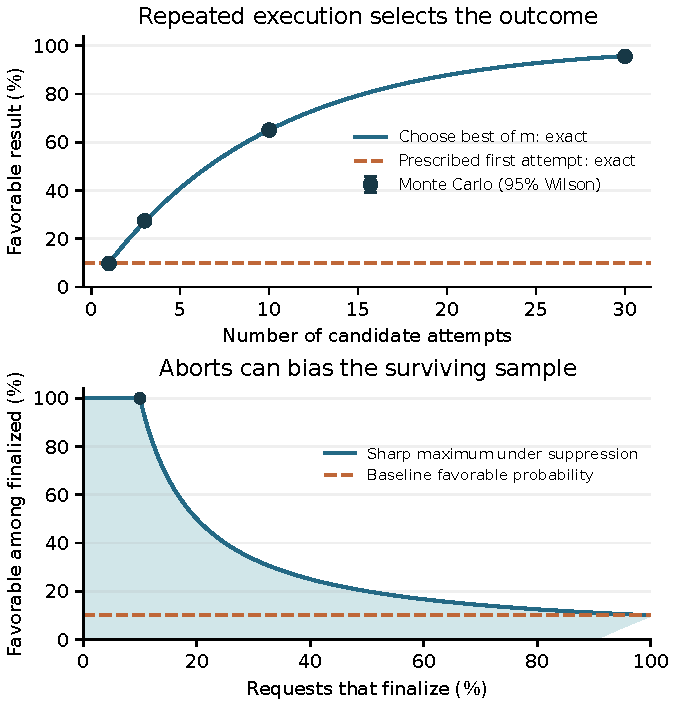
\includegraphics[width=\linewidth]{figures/selection-integrity.pdf}
\caption{Selection integrity at baseline favorable probability 0.1. Top: exact retry advantage and Monte Carlo estimates; intervals are pointwise 95\% Wilson intervals. Bottom: the sharp interval obtainable by outcome-dependent suppression at each completion rate. The upper boundary reaches 100\% when only favorable requests complete. The shaded region is an analytic bound, not an empirical confidence interval.}
\label{fig:selection}
\end{figure}

An exhaustive eight-element probability-space check evaluates 65,280 event/selection pairs with no violation of either sharp conditional bound. A separate deterministic toy computation repeats 10,000 fixed requests thirty times each: all 300,000 re-executions preserve their initial result. This checks the restart construction; it is not evidence that a hosted LLM API or GPU kernel is deterministic. Certificate and attempt tests also preserve the accepted hidden-restart counterexample for a slot policy that does not fix execution randomness.

\subsection{Measured AVM costs}
\label{sec:avm}

The cryptographic kernel is compiled with PuyaPy 5.7.1, optimization level 2, targeting AVM 11, and executed on native go-algorand 5.0.3 (commit \texttt{2dc9524e}) with private consensus v42. It checks stored context and count, fixed-width indices, proof length, payload and leaf hashes, every sibling, the root wrapper, and optionally an Ed25519 signature on the stored result/trace projection. The approval program is 624 bytes; the clear program is 2 bytes. The measured profile uses power-of-two counts; padded trees are covered by the independent off-chain conformance study.

\begin{table}[t]
\centering\small
\caption{Complete cryptographic verification kernel, all indices. Group costs include required 29-unit budget calls; each reported group also includes one zero-value self-payment. Fees are base fees before argument-size surcharges.}
\label{tab:avm}
\begin{tabular}{llrrr}
\toprule
Slots & Method & Main call & Worst group & App calls / fee (ALGO)\\
\midrule
4 & Membership & 384--386 & 386 & 1 / 0.002\\
16 & Membership & 540--544 & 544 & 1 / 0.002\\
64 & Membership & 696--702 & 731 & 2 / 0.003\\
4 & Signed & 2,345--2,347 & 2,434 & 4 / 0.005\\
16 & Signed & 2,501--2,505 & 2,592 & 4 / 0.005\\
64 & Signed & 2,657--2,663 & 2,750 & 4 / 0.005\\
\bottomrule
\end{tabular}
\end{table}

The study checks all 84 positions across the three sizes for both methods, giving 168 index/method measurements. Another 24 accepted groups vary payload sizes from 256 to 4,096 bytes; 18 use actual reference trace records. Those 42 groups were submitted and confirmed, without extra-budget simulation overrides. Forty-five negative controls test malformed proofs, state/context mismatch, signatures, and actual resource limits. A fresh-ledger reproduction agrees on opcode costs and acceptance behavior; transaction identities, rounds, and RPC timings need not match.

The precise result matters. A 64-leaf leftmost path costs 702 units and needs a second application call; quoting only the 696-unit rightmost path would hide that boundary. An application call contributes 700 units to the pool, while a payment contributes none. A verifier grouped with fifteen payments still lacks the signature budget. The signed path includes a 1,900-unit \texttt{ed25519verify\_bare} and its additional message hash \cite{algorandopcodes2026,algorandcosts2026}.

For this tree encoding, the membership hash-only lower bound is
\[
35\bigl(\lceil\log_2 n\rceil+3\bigr),
\]
including payload hashing, the leaf envelope, and root wrapper. It is 175, 245, and 315 units at 4, 16, and 64 leaves. Table~\ref{tab:avm} includes the parsing of binary arguments, bounds, loop, state, and comparison work omitted by that lower bound. It still does not include blueprint semantic replay, registration, TEE document verification, or the full reveal/settlement state machine.

The whole-trace single-buffer hash baseline costs 71 units for the 2,166- and 3,356-byte traces. The 8,156-byte trace exceeds the individual 4,096-byte argument/stack limit; a streaming whole-trace baseline is feasible in principle but is not measured here. Consensus v42 permits larger combined arguments with a fee surcharge of 0.1 microAlgo per byte above 2,048, rounded up at the group level, while retaining the individual-value limit \cite{algorandfees2026}. Thus a 4,096-byte leaf succeeds with a surcharge, whereas a payload plus proof can exceed the free argument allowance even when the payload alone fits. Fees buy argument capacity, not opcode budget.

The test application's setup reserves 378,500 microAlgo of minimum balance for one integer and five byte-valued global slots plus the application base. That is neither a per-proof fee nor an estimate of a complete market's storage requirement. The private-ledger measurements establish practical compact verification under pinned rules. Public-chain latency, production publication storage, and complete-market costs remain measurements for the deployment study.

\FloatBarrier
\section{Economic Fallback and Product Validation}
\label{sec:product}

Verified execution changes what a challenger must establish. It does not remove the need to pay for discovering and adjudicating faults. The companion resolution paper derives funded inspection conditions and exposure-scaled deterrence under explicit coverage and adjudication assumptions \cite{trustexplicit2026}. Those conditions replace a universal fixed bond or fixed challenge-window recommendation.

The relevant verification cost is a sum: retrieving the account, locating a questionable step, authenticating the evidence, checking its semantics, and submitting or defending the challenge. A Merkle proof can reduce the authenticated evidence sent to the contract. It need not reduce the time needed to discover the bad step. Attestation can reduce the need to distrust every claimed local transition. It does not make a false source report, an ambiguous question, or a poor model judgment disappear.

The practical proposition is still strong: blueprints define the rules; traces pin the account; execution evidence narrows substitution; request rules constrain selection; and funded challenges handle the residual. The market's exposure and the remaining failure modes determine which layers are worth buying.

\subsection{Why question.market is a useful test bed}

question.market controls the components that need to be varied independently: market creation, blueprint publication, execution requests, evidence presentation, runner selection, challenges, and final settlement. This makes it a suitable platform for a causal study of execution assurance while holding the question, source snapshot, and adjudication path fixed. The current implementation need not match the research protocol for the paper to stand on its own; a test deployment must identify exactly which revision and assurance profile it implements.

Every trial must retain a request record before outcome production, including market exposure, blueprint/snapshot commitments, committee and dependency map, seed and sampling policy, start/expiry times, every permitted attempt, failures, publication events, challenges, and adjudication. An absent result is an observation. Measuring only finalized markets would erase the selective-abort effect established in Section~\ref{sec:selection}.

A useful first comparative study has three interfaces over the same case material: a complete canonical trace with a whole-trace hash; the same trace with Merkle openings and node-specific tools; and the same tools with request-bound signed or genuinely attested receipts. Random assignment of interface and fault condition should measure diagnostic correctness, false accusations, time to first correct diagnosis, bytes retrieved, transaction cost, and missed deadlines. Keep source falsity separate from transition fabrication: stronger execution evidence is not expected to repair a false source by itself.

The independent unit is the question/snapshot/request or independently sampled fault scenario, not every node or every repeated verifier click. Pair interfaces on matched cases and cluster uncertainty by that unit and, where appropriate, operator. Determine sample size from a declared primary effect and a blinded pilot estimate of variance or paired discordance. Do not infer a population false-acceptance rate from this paper's designed rejection vectors. For genuinely independent representative Bernoulli trials with zero failures, the one-sided 95\% upper bound is $1-0.05^{1/N}$; designed attack cases and correlated repeats do not satisfy that sampling premise.

A subsequent hardware experiment should launch independently built images, verify source-to-measurement reproducibility, perform real remote-attestation registration, terminate TLS within the measured boundary, and inject host delay, false plaintext, stale objects, key revocation, restarts, and coordinator censorship. Record image/build hashes, hardware and cloud configuration, latency distributions, boot and quote times, resource use, and complete protocol costs. The present prototype gives that experiment an exact acceptance oracle instead of an informal expectation of what ``verified'' means.

\section{Directions Worth Pursuing}
\label{sec:directions}

\textbf{Proof-carrying subgraphs.} The most useful ZK question is not whether an entire open-ended resolver can be proved today. It is which deterministic transformations are cheap enough to prove and which boundary inputs still need source authentication, attestation, or judgment. The composition theorem supplies a common interface. Compare replay, a general zkVM, and specialized proofs on the same pinned source/extraction/branch workload. Report prover time, verifier cost, proof size, memory, and the exact trusted input boundary. A remote API receipt is not a proof of the provider's model; a model proof is not a proof that its answer is true.

\textbf{A public execution-request log.} Release transparency makes the permitted software inspectable. An analogous public request-and-attempt record makes selection inspectable. The strongest near-term experiment combines a frozen request, independently generated randomness, deterministic repeated execution, and permissionless submission of the same valid result. Compare its favorable-result rate \emph{and} completion rate with unconstrained retrying. Hardware protects a run; the authoritative log controls which runs count.

\textbf{Dependency-aware committee selection.} The important unit of diversity is a trust dependency, not a public key. A compiler can expose shared vendors, registrars, builds, provider accounts, and upstream data. The quorum policy can then be checked against explicit compromise and outage sets before a market opens. The exact covering and intersection calculations in this paper are small enough to do at creation time. Their inputs still need evidence and governance; invented independence is worse than a visible single dependency.

\textbf{A funded verification budget.} A market can declare the maximum evidence size, necessary disclosure policy, and expected cost of checking its workflow. The execution measurements then feed the inspection incentives of the companion paper. The falsifiable question is whether compact challenges and stronger provenance reduce the reward needed to sustain reliable checking at equal market exposure. That requires measuring discovery and adjudication work, not merely counting hashes.

\section{Scope of the Evidence}

The paper provides proofs under explicit cryptographic and behavioral assumptions, an executable bounded workflow profile, adversarial vectors, cross-language commitment checks, a committee/attempt state model, and real compiled AVM measurements on a private test ledger. The AVM verifier authenticates records and a signed receipt projection. It does not implement the complete market, general JSON semantics, Nitro certificate appraisal, the full publication service, or a production dispute economy.

The committee model's public HMAC test fixtures exercise authentication and policy state transitions; they are not public-key security or hardware measurements. Source fixtures exercise actual RSA signature verification with intentionally public test keys. The AVM signed path exercises actual Ed25519 verification. None of those experiments establishes physical enclave isolation, real vendor independence, reproducible Nitro images, or the truth of a provider's report. Those are precisely the boundaries assigned to the next deployment study.

The source/add/branch/terminal grammar is a complete reference profile, not a claim to cover every blueprint. Large blobs, joins, retries inside a graph, confidential evidence, and asynchronous human judgments require additional bounded semantics and publication rules. The general composition theorem applies when those local rules and their checkers satisfy its premises. The runtime cannot inherit the theorem merely by naming a new node type.

\section{Conclusion}

A market should not stop at declaring how it will resolve. It should carry evidence that its declared decision program was followed, that the counted execution was authorized, and that the evidence was available in time to challenge.

The two-axis model keeps execution assurance separate from the kind of judgment on which settlement depends. The trace protocol makes the account complete and selectively challengeable. The common-result certificate makes independent execution meaningful without demanding identical run metadata. The attempt policy exposes a failure that attestation alone cannot fix: selecting the result after seeing it. The compiled verifier measurements show that compact checking is practical, while locating the actual budget and publication costs.

The resulting architecture is stronger because its boundaries are executable. A false transition, missing record, substituted request, invalid committee, or withheld attempt becomes a specific protocol event. Source truth and judgment remain visible dependencies, with funded disputes where they belong. Markets should progressively improve evidence that the committed program actually ran. This paper supplies the commitments, proofs, and experiments needed to make that progression concrete.

\appendix
\section{Reproduction and Acceptance Boundaries}

The source and public evidence are in the \href{https://github.com/qmrkt/research}{research repository}, directory \path{03-verified-execution}. \path{PROTOCOL.md} specifies exact objects, encodings, tree rules, and the bounded semantic/publication profile. \path{QUORUM.md} specifies committee, dependency, and attempt policies. \path{REPRODUCIBILITY.md} maps claims to saved artifacts and commands. The final revision manifest records file hashes. Earlier paper PDFs remain recoverable in Git history.

The installed Python research package uses the standard library; the independent commitment verifier uses Node.js. The clean-wheel check installs outside the checkout and runs all three papers' tests without injecting source paths. Optional matplotlib regenerates the selection figure from saved observations and the proved conditional-selection bounds. The AVM harness has separately pinned compiler/SDK requirements and creates a fresh disposable private ledger; it neither resets a product network nor spends live-network funds.

\begin{table}[h]
\centering\small
\caption{What each executable check establishes. Passing one row does not imply the properties in later rows.}
\renewcommand{\arraystretch}{1.12}
\begin{tabularx}{\linewidth}{p{0.25\linewidth}YY}
\toprule
Check & Accepted fact & Remaining check\\
\midrule
Canonical encoding & One permitted byte representation & Exact schema and semantic validity\\
Merkle opening & Bytes at a bound count/index/context & Whether those bytes describe valid execution\\
Complete replay & Correct bounded computation on fixed authenticated inputs & Historical invocation and source truth\\
Publication gate & All required bytes disclosed before the checking window & Attentive checking and semantic acceptance\\
Runner receipt & Authorized key endorsed bound evidence/result & Approved program and key custody\\
Attestation appraisal & Declared hardware evidence meets an appraisal policy & Correct code, source truth, and persistent attempt control\\
Quorum certificate & Enough eligible distinct identities endorse one result & Fault assumptions, dependency diversity, and availability\\
Attempt completion & Required public slots follow the declared policy & Hidden resampling unless fixed execution prevents it\\
\bottomrule
\end{tabularx}
\end{table}

Hash, commitment, and signature security are assumptions of the proofs, not claims inferred from a finite number of tests. Conformance vectors preserve honest controls and attacks that correctly remain possible: authentic false inputs, shared-dependency compromise, hidden stochastic restarts, selective abort, and unchecked semantic fraud in the optimistic publication profile. Those cases identify the next required layer instead of disappearing from the results.

\section*{Acknowledgments}
This manuscript was developed with large language model assistance for protocol and experiment implementation, mathematical formalization, literature review, and critical review of drafts. The underlying mechanism design, thesis, research direction, and earlier prototypes are the author's own.
\begin{thebibliography}{99}

\bibitem{trustexplicit2026}
Andrei Savin.
\newblock \emph{Trust-Explicit Resolution for Prediction Markets: Declared Logic, Verifiable Traces, and Dispute Economics}.
\newblock Working paper, 2026.
\newblock Available at \url{https://question.market/research/trust-explicit-resolution.pdf}.

\bibitem{towncrier2016}
Fan Zhang, Ethan Cecchetti, Kyle Croman, Ari Juels, and Elaine Shi.
\newblock \emph{Town Crier: An Authenticated Data Feed for Smart Contracts}.
\newblock In \emph{Proceedings of the 2016 ACM SIGSAC Conference on Computer and Communications Security}, pages 270--282, 2016.

\bibitem{ekiden2019}
Raymond Cheng, Fan Zhang, Jernej Kos, Warren He, Nicholas Hynes, Noah Johnson, Ari Juels, Andrew Miller, and Dawn Song.
\newblock \emph{Ekiden: A Platform for Confidentiality-Preserving, Trustworthy, and Performant Smart Contracts}.
\newblock In \emph{Proceedings of the 2019 IEEE European Symposium on Security and Privacy}, pages 185--200, 2019.

\bibitem{deco2020}
Fan Zhang, Sai Krishna Deepak Maram, Harjasleen Malvai, Steven Goldfeder, and Ari Juels.
\newblock \emph{DECO: Liberating Web Data Using Decentralized Oracles}.
\newblock In \emph{Proceedings of the 2020 ACM SIGSAC Conference on Computer and Communications Security}, pages 1919--1938, 2020.

\bibitem{tlsnotary}
TLSNotary Project.
\newblock \emph{Notarization}.
\newblock Documentation, accessed 2026.
\newblock \url{https://tlsnotary.org/docs/protocol/notarization/}.

\bibitem{chainlinkcc}
Lorenz Breidenbach, Alex Coventry, Siam Hussain, Yan Ji, Dahlia Malkhi, Christian M\"{u}ller, Gregory Neven, Chrysoula Stathakopoulou, Philipp Schindler, and Pawe{\l} Sza{\l}achowski.
\newblock \emph{Chainlink Confidential Compute}.
\newblock White paper, November 2025.
\newblock \url{https://research.chain.link/confidential-compute.pdf}.

\bibitem{rfc8785}
Anders Rundgren, Bret Jordan, and Samuel Erdtman.
\newblock \emph{JSON Canonicalization Scheme (JCS)}.
\newblock RFC 8785, Internet Engineering Task Force, 2020.
\newblock \url{https://www.rfc-editor.org/rfc/rfc8785}.

\bibitem{nitrodocs}
Amazon Web Services.
\newblock \emph{Verifying the root of trust}.
\newblock AWS Nitro Enclaves User Guide, accessed 2026.
\newblock \url{https://docs.aws.amazon.com/enclaves/latest/user/verify-root.html}.

\bibitem{algorandcosts2026}
Algorand Foundation.
\newblock \emph{Smart Contract Costs \& Constraints}.
\newblock Developer documentation, accessed 2026.
\newblock \url{https://dev.algorand.co/concepts/smart-contracts/costs-constraints/}.

\bibitem{arbitrum2018}
Harry Kalodner, Steven Goldfeder, Xiaoqi Chen, S. Matthew Weinberg, and Edward W. Felten.
\newblock \emph{Arbitrum: Scalable, private smart contracts}.
\newblock USENIX Security, 2018.
\newblock \url{https://www.usenix.org/conference/usenixsecurity18/presentation/kalodner}.
\bibitem{rats2023}
Henk Birkholz, Dave Thaler, Michael Richardson, Ned Smith, and Wei Pan.
\newblock \emph{Remote ATtestation procedureS (RATS) Architecture}.
\newblock RFC 9334, January 2023.
\newblock \url{https://www.rfc-editor.org/rfc/rfc9334}.
\bibitem{pcc2026}
Apple.
\newblock \emph{Release Transparency}.
\newblock Private Cloud Compute Security Guide, accessed October 2026.
\newblock \url{https://security.apple.com/documentation/private-cloud-compute/releasetransparency}.
\bibitem{aex2026}
Yongjie Guan.
\newblock \emph{AEX: Non-Intrusive Multi-Hop Attestation and Provenance for LLM APIs}.
\newblock arXiv:2603.14283v1, March 2026.
\newblock \url{https://arxiv.org/abs/2603.14283v1}.
\bibitem{aep2026}
Anton Sokolov.
\newblock \emph{Hardware-rooted attestation for AI-agent evidence: composing IETF RATS with action evidence packages}.
\newblock arXiv:2608.00801v1, August 2026. Technical note; software-TPM demonstration.
\newblock \url{https://arxiv.org/abs/2608.00801v1}.
\bibitem{zkllm2024}
Haochen Sun, Jason Li, and Hongyang Zhang.
\newblock \emph{zkLLM: Zero Knowledge Proofs for Large Language Models}.
\newblock ACM CCS, 2024; author version arXiv:2404.16109.
\newblock \url{https://arxiv.org/abs/2404.16109}.
\bibitem{teerex2026}
Sadegh Keshavarzi, Gregory Chockler, and Alexey Gotsman.
\newblock \emph{TEE Is Not a Healer: Rollback-Resistant Reliable Storage}.
\newblock DISC 2025; extended version arXiv:2505.18648v3, April 2026.
\newblock \url{https://arxiv.org/abs/2505.18648v3}.
\bibitem{nitropcr2026}
Amazon Web Services.
\newblock \emph{Cryptographic attestation}.
\newblock AWS Nitro Enclaves User Guide, accessed October 2026.
\newblock \url{https://docs.aws.amazon.com/enclaves/latest/user/set-up-attestation.html}.
\bibitem{nitrokms2026}
Amazon Web Services.
\newblock \emph{Connect an enclave with AWS KMS for cryptographic attestation and secrets management}.
\newblock AWS Nitro Enclaves User Guide, accessed October 2026.
\newblock \url{https://docs.aws.amazon.com/enclaves/latest/user/connect-enclave-kms.html}.

\bibitem{algorandopcodes2026}
Algorand Foundation.
\newblock \emph{AVM Opcodes}.
\newblock Developer documentation, accessed October 2026.
\newblock \url{https://dev.algorand.co/reference/algorand-teal/opcodes/}.
\bibitem{algorandfees2026}
Algorand Foundation.
\newblock \emph{Transaction Fees}.
\newblock Developer documentation, accessed October 2026.
\newblock \url{https://dev.algorand.co/concepts/transactions/fees/}.
\end{thebibliography}

\end{document}
